\documentclass[10pt, a4paper]{article}
\usepackage[T1]{fontenc}
\usepackage[utf8]{inputenc}
\usepackage{url}

\usepackage[english]{babel}
\usepackage{blindtext}

\usepackage{float} %To edit float behaviour
\usepackage{graphicx} %To include images
\usepackage[leftcaption]{sidecap} %Side captions %options: outercaption, innercaption, leftcaption, rightcaption

% \usepackage[slc=on]{caption} %for subfloats
% \usepackage{subcaption}
\usepackage{threeparttable}

\usepackage{subfig}

\usepackage{hyperref}
\setcounter{lofdepth}{2}

\begin{document}
\listoffigures
\newpage
\section{Different ways to include images}


\begin{figure}[h]
\centering
  \includegraphics[width=0.5\textwidth]{gull_picture}
\end{figure}

\begin{figure}[h]
  \centering
      \reflectbox{\includegraphics[width=0.5\textwidth]{pics/gull_picture}}
  \caption{A picture of the same gull
           looking the other way!}
\end{figure}
\newpage

% \begin{figure}[h]
%         \centering
%         \begin{subfigure}[t]{0.3\textwidth}
%                 \centering
%                 \includegraphics[width=\textwidth]{gull_picture}
%                 \caption*{A gull}
%                 \label{fig:gull}
%         \end{subfigure}%
%         ~ %add desired spacing between images, e. g. ~, \quad, \qquad etc.
%           %(or a blank line to force the subfigure onto a new line)
%         \begin{subfigure}[t]{0.3\textwidth}
%                 \centering
%                 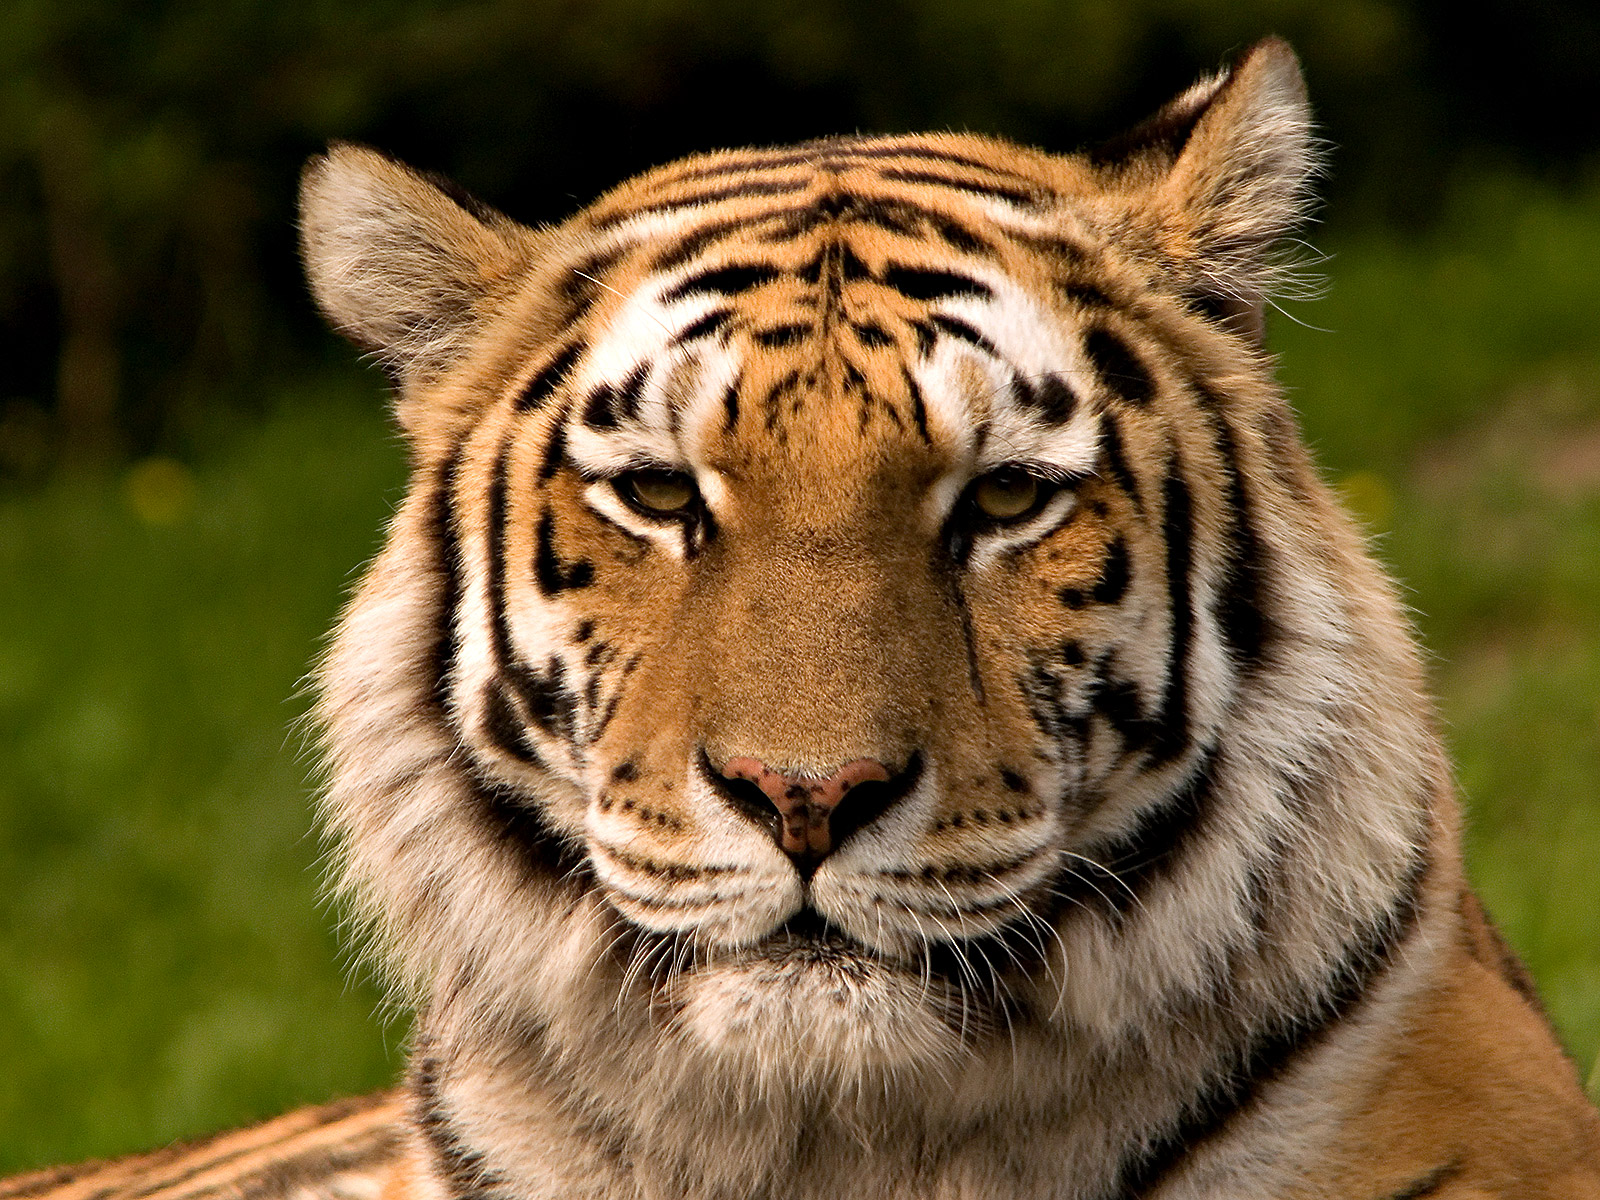
\includegraphics[width=\textwidth]{tiger_picture}
%                 \caption{A tiger}
%                 \label{fig:tiger}
%         \end{subfigure}%
%         ~ %add desired spacing between images, e. g. ~, \quad, \qquad etc.
%           %(or a blank line to force the subfigure onto a new line)
%         \begin{subfigure}[t]{0.3\textwidth}
%                 \centering
%                 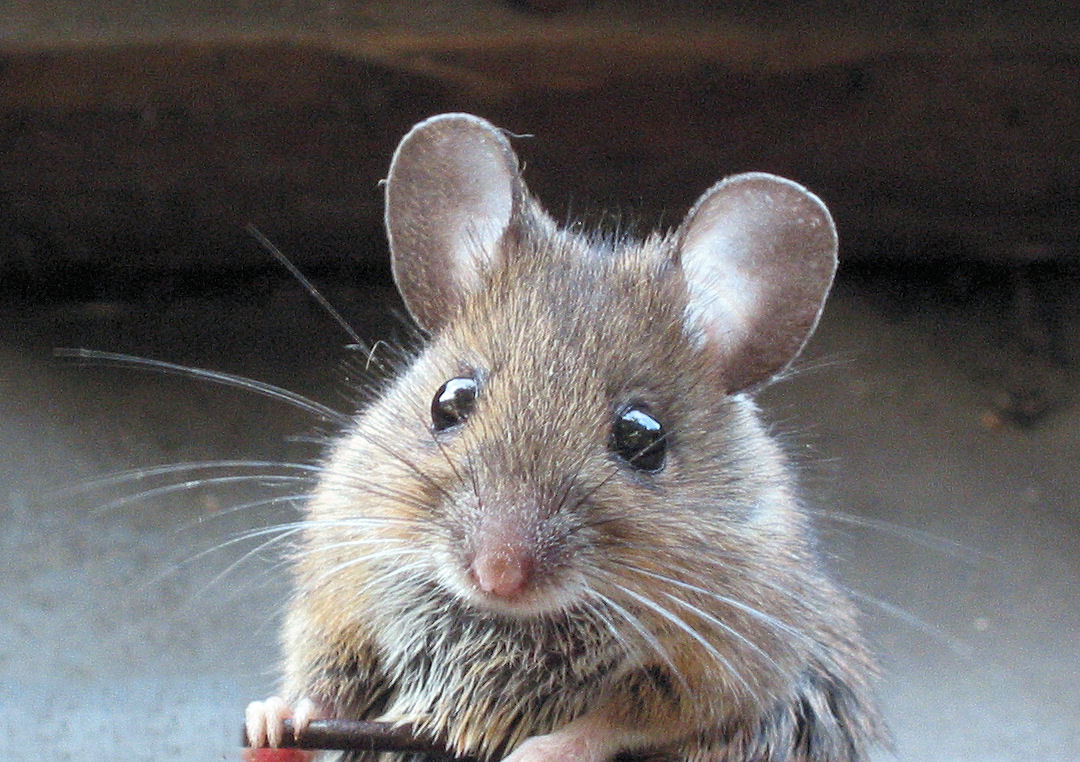
\includegraphics[width=\textwidth]{mouse_picture}
%                 \caption{A mouse}
%                 \label{fig:mouse}
%         \end{subfigure}
%         \caption{Pictures of animals}\label{fig:animals}
% \end{figure}

\begin{figure}
\centering
  \subfloat[Minicaption][Long caption]{\includegraphics[width=0.3\textwidth]{gull_picture}}~
  \subfloat[Minicaption][Long caption]{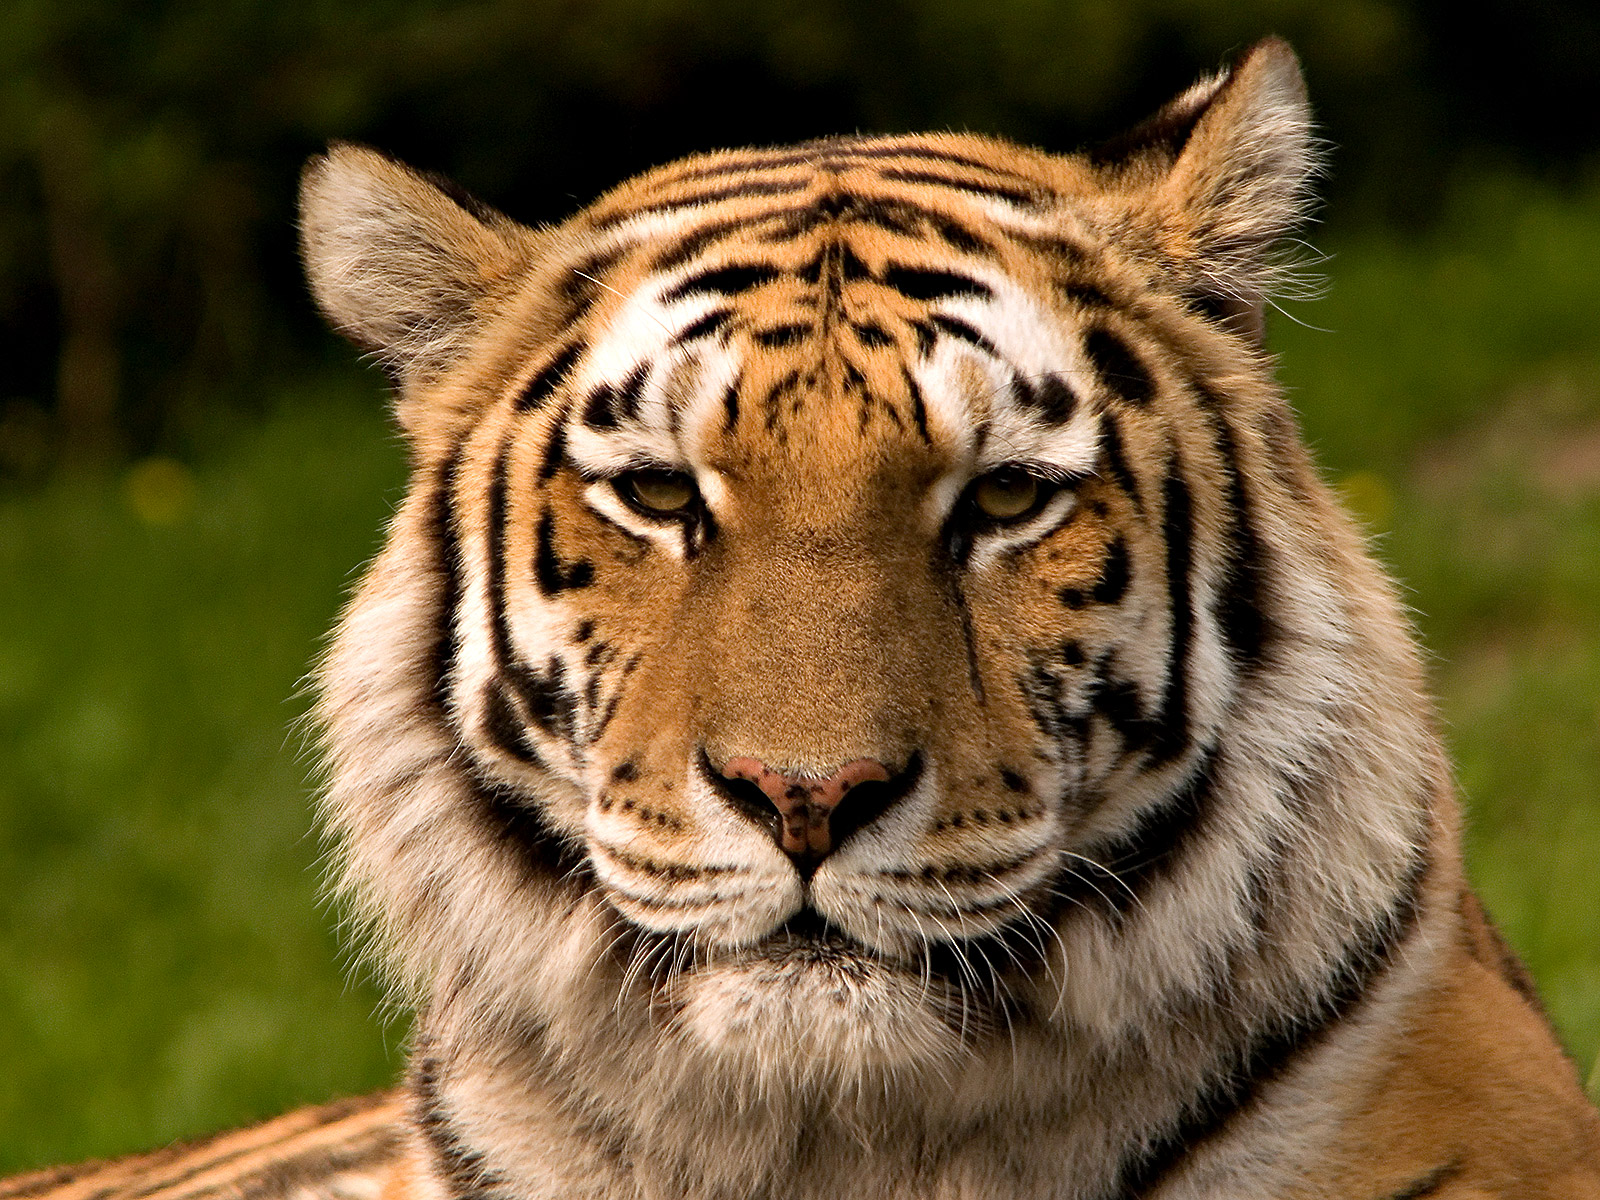
\includegraphics[width=0.3\textwidth]{tiger_picture}}~
  \subfloat[Minicaption][Long caption]{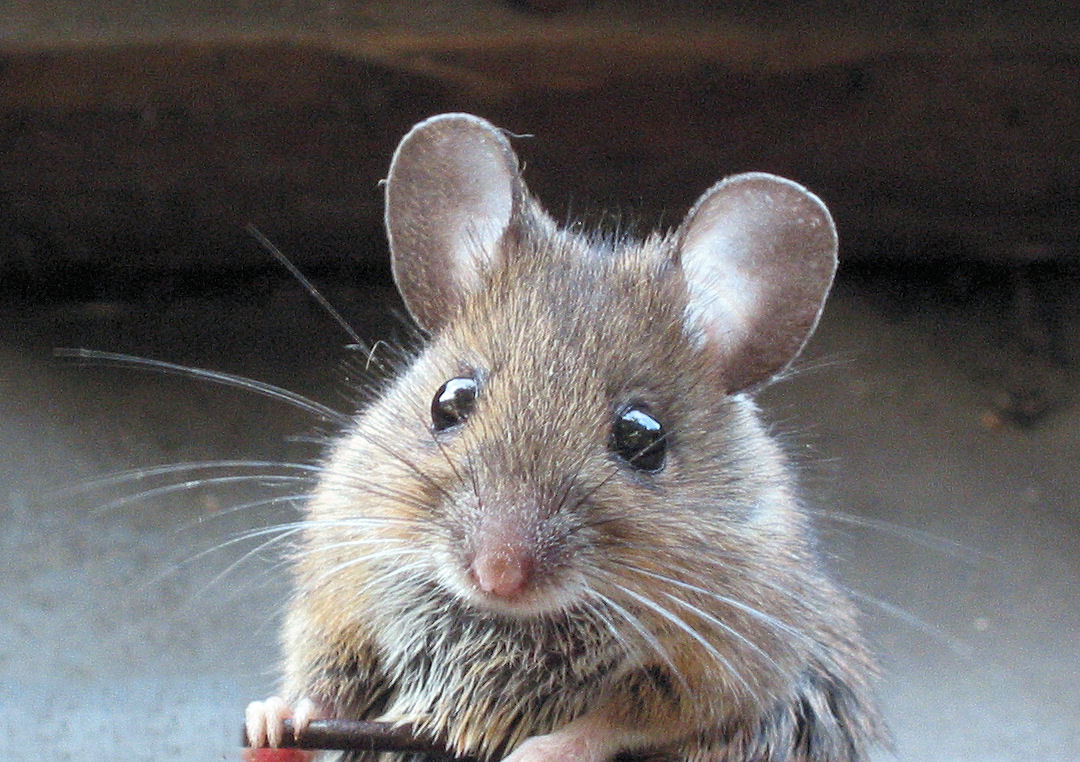
\includegraphics[width=0.3\textwidth]{mouse_picture}}

  \subfloat[Minicaption][Long caption]{\includegraphics[width=0.3\textwidth]{gull_picture}}~
  \subfloat[Minicaption][Long caption]{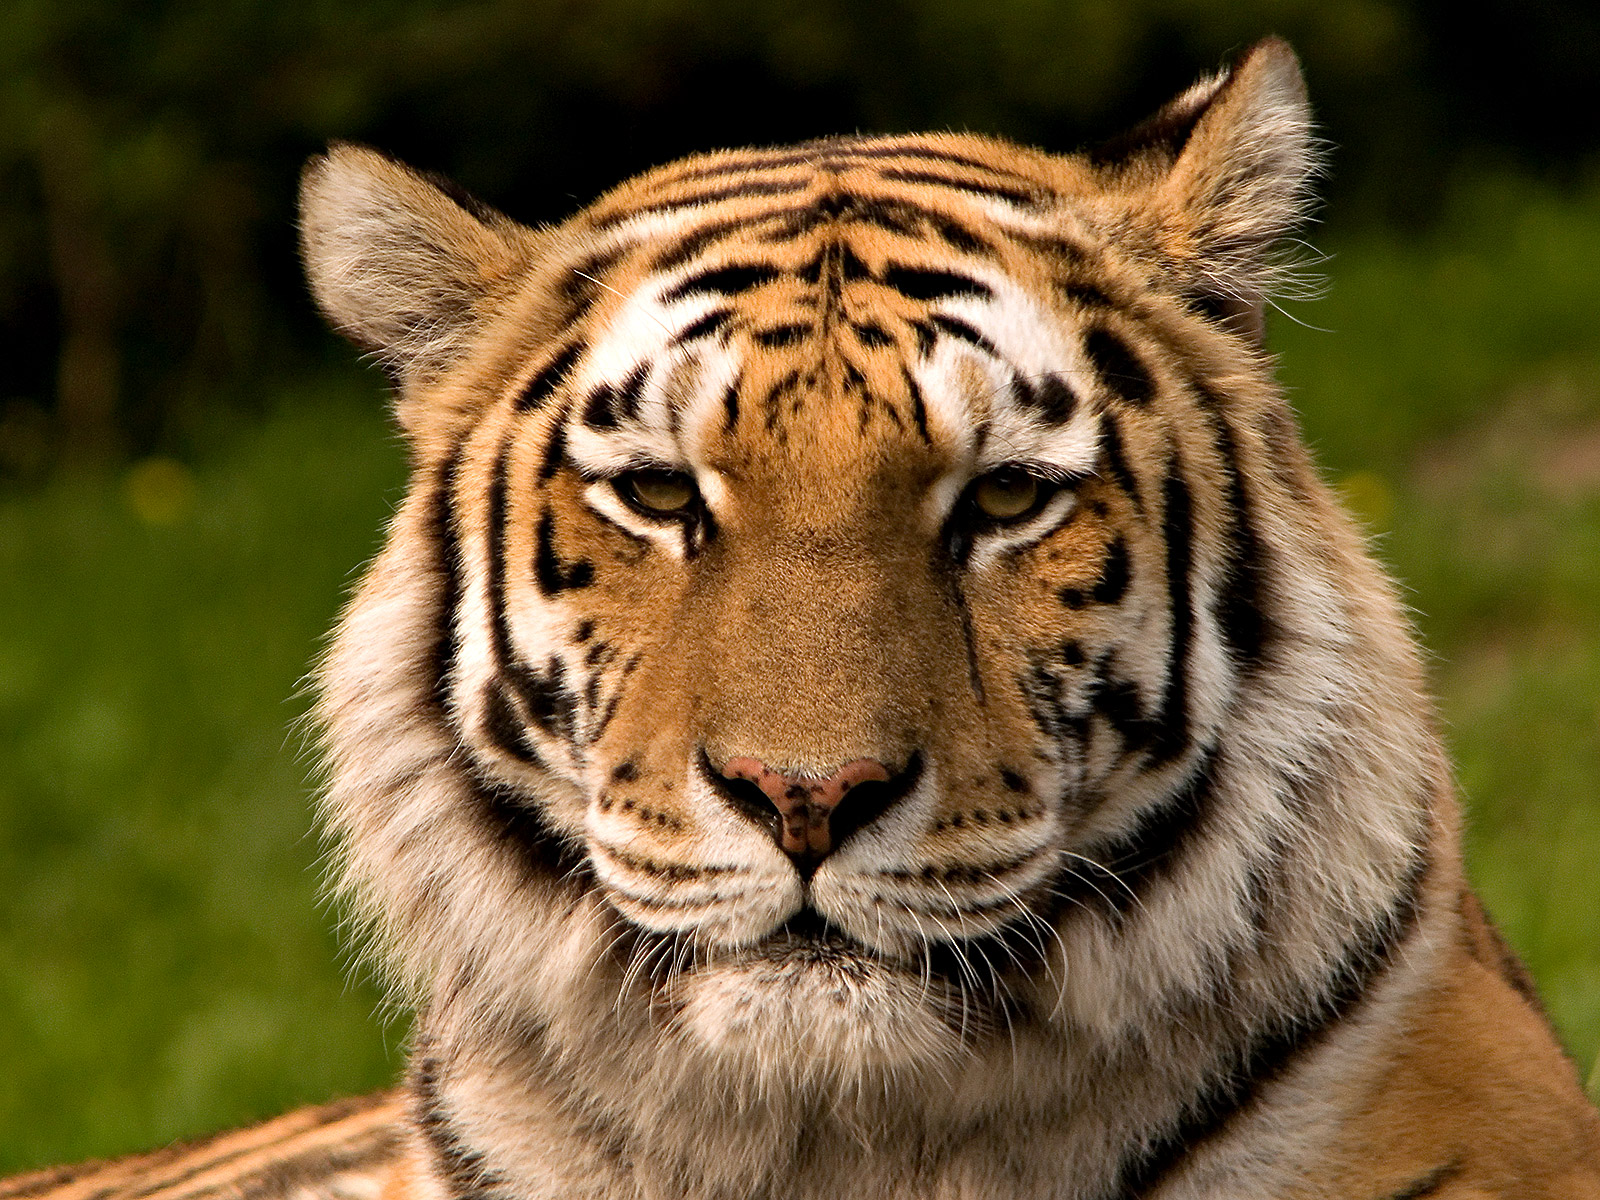
\includegraphics[width=0.3\textwidth]{tiger_picture}}~
  \subfloat[Minicaption][Long caption]{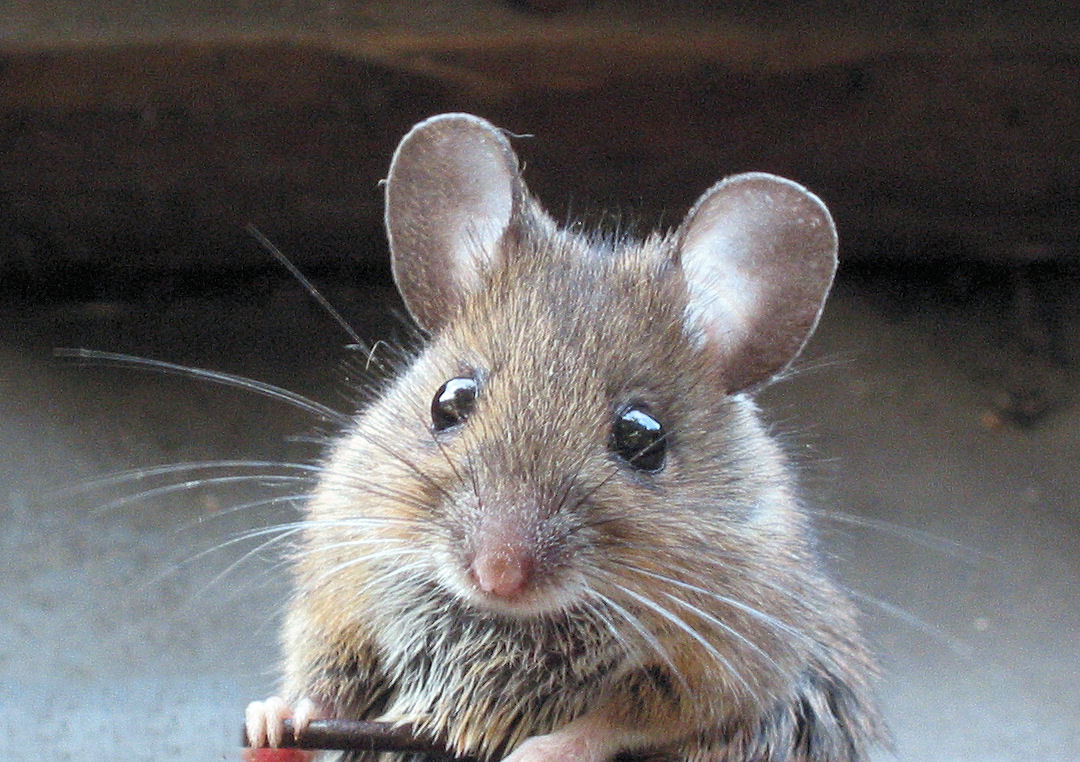
\includegraphics[width=0.3\textwidth]{mouse_picture}}  
  \caption{Overview}
\end{figure}


\begin{SCfigure}[][h] %[relwidth of caption][float]
  \includegraphics[width=0.5\textwidth]%
    {giraff_picture}% picture filename
  \caption{caption text}
\end{SCfigure}



{
\floatstyle{boxed}
\restylefloat{figure}\restylefloat{table}
\begin{figure}[h]

A figure can also contain just text!

\blindtext
\caption{\blindtext \label{fig:formeln}}
\end{figure}
}


\section{Labels in Captions}

A remark on labels in captions:
\begin{quote}
If you want to label a figure so that you can reference it later, you have to add the label after the caption (inside seems to work in \LaTeXe) but inside the floating environment. If it is declared outside, it will give the section number.\end{quote}

\noindent\url{http://en.wikibooks.org/wiki/LaTeX/Floats,_Figures_and_Captions}
\end{document}
